\chapterimage{TA.pdf}
\chapterimagecaption{\textit{The Night Before The Exam
} (1895) by Leonid Pasternak}

\chapter{TAing}

    
\section{What is a TA?}

A Teaching Assistant (TA) is a graduate student who assists an instructor in conducting a course. Their duties include but are not limited to teaching concepts, organizing tutorials and office hours, aiding with labs, grading assignments and exams, and invigilation. All TAs are members of the \href{https://tsum-stsem.ca/}{ Teaching Support Union at McGill (TSUM)}, formerly known as the Association of Graduate Students Employed at McGill (AGSEM). \\

%\begin{plainbox}
%\noindent \textbf{\sffamily Who can become a TA?} \\
%All \textbf{graduate students} at McGill are eligible to apply for a TAship. 
%\end{plainbox}

\noindent \textbf{\sffamily How do I become a TA?} \index{Teaching Assistantship!Application}\\
All graduate students have the right to apply for a TAship and they will be hired after submitting an application form to a department
(Hiring Unit). You can apply for and work TA positions in departments other than your own. There is only one application process per term for each Hiring Unit. You'll receive an email from the Graduate Program Coordinator (GPD) when the application is live. TA positions are  posted on Workday by: \vspace{5pt}
\begin{itemize}
    \item For Fall courses: 3rd Monday of May,
    \item For Winter courses: 3rd Monday of October,
    \item For Summer courses: 2nd Monday of March.
\end{itemize}

\begin{plaincorollary}
Students need to apply as an external candidate on Workday for the Fall postings since they won't have access to their work email. All postings will be up for at least 14 calendar days and you will be notified withing 35 days of the application deadline. 
\end{plaincorollary}


\noindent \textbf{\sffamily What does a TA contract look like?} \index{Teaching Assistantship!Contract}
\begin{plainexercise}
  All TAs work for 90 hours per semester. The maximum size of a TA position is 180 hours per academic year. The rate of pay for 2026-27 is \textbf{\$38.46 per hour} so a student is eligible for \$6922.8 before taxes for the combined year 2026-27 (Fall + Winter).   
\end{plainexercise}
Our \href{https://tsum-stsem.ca/documents/Simplified%20CA%20August%202024.pdf}{Collective Agreement (CA)} is set to expire on July 31, 2027 after which a new contract will take its place. A CA is a written legal contract between an employer (McGill) and the union that outlines the rules and conditions for the workers (TAs). 

TA salaries are paid \textbf{biweekly}, and the pay schedule is available on your Workday dashboard and on \href{https://www.mcgill.ca/hr/files/hr/2026_salaried_pay_calendar.pdf}{McGill's website.} Each payday is for approximately 12 hours (except for the first one) so you can expect a recurring payment of roughly \$420 every 2 weeks. \\

\noindent \textbf{\sffamily What happens after I accept my offer?} \\
You must accept a TA offer via the Workday portal within \textbf{7 days} of receiving an
offer letter. There are exceptions to the 7 day rule due to documented
illness. If you are offered a position that is later withdrawn, you must be offered a vacant position of at least the same size. After accepting your offer, at the beginning of the semester, you must: 

\begin{enumerate}
    \item \textbf{Complete the onboarding on Workday.} This involves verifying your personal information and checking your tax contributions such as RRSP or TFSA. \\

    \item \textbf{Fill the \href{https://tsum-stsem.ca/members/membership-forms/}{Union Membership Form}} for full union membership. All TAs are considered members of the union, regardless of whether they fill the membership form. However, if the visible strength of the union falls below a certain number, the union may cease to exist so it is highly recommended.\\

    \item \textbf{Meet with the instructor} to discuss your tasks and divide them between you and other TAs. The instructor should also provide you access to the myCourses page of the course and possibly Crowdmark if they plan on using it for grading. \\

    \item \textbf{Fill out the \href{https://www.mcgill.ca/hr/files/hr/agsem_ta_workload_form_en-fillable.pdf}{Workload Form.}} It is a very useful tool that provides a structured approach to
    formally negotiate your workload, maintain a detailed record of your hours, and request additional hours if needed. 

    \begin{plainbox}
        Students must ensure that they don't work more than the \textbf{90 hours} per semester limit. If the course instructor forces you to go over this limit, contact your \href{https://tsum-stsem.ca/contact/}{ \underline{department delegate}} immediately. 
    \end{plainbox}

    \item \textbf{Access your work email}. Students should now be able to access their work email that ends in @mcgill.ca. This email can be used for all communications between students or the course instructor. If you are new student and have not had a @mcgill.ca before, you'd need to set it up via Outlook like you did for your personal email. \\

    \item \textbf{Review your workload form} at the halfway mark of the term and meet with the instructor to review your performance and hour allocation. The midterm review is highly recommended as it helps to adjust the distribution of hours if enrollment has fluctuated or if you feel you need more time for certain tasks. \\
\end{enumerate}



\noindent \textbf{\sffamily Do I have any job security as a TA?} \index{Teaching Assistantship!Priority Pool}\\
TAs are entitled to preferential hiring based on seniority. This is called the
\textbf{Priority Pool} (PP). Every semester, a department must assign any available TA positions to applicants with priority, starting with the highest level of priority. Priority declines as following:

\begin{plaindefinition}
    \begin{itemize}
        \item Fourth-year PhD
        \item Third-year PhD
        \item Second-year PhD
        \item First-year PhD
        \item Second-year Master's
        \item First-year Master's
        \item Fifth-year PhD
    \end{itemize}
\end{plaindefinition}

\noindent You enter the PP once you accept a job in a department and the length of time you have in the PP is determined by the date of your initial enrolment. For example, a PhD4 applicant who has never been a TA in that department before \textbf{does not} have priority. Applicants who are more advanced in their programs may still have priority if they receive extensions to their PP entitlement, for things like field work or maternity leave.

\noindent\textbf{\color{ocre} Note:} Applicants with PP status are given priority for a TA position, but not for
the specific TA position that they want. 

\subsection{What is TSUM?} \index{TSUM}
All TAs are represented by a labour union, the Teaching Support Union at McGill (TSUM). The union changed its name very recently, in April 2026, from Association of Graduate Students Emplyeed at McGill (AGSEM) to TSUM. Hence we'll refer to it as TSUM throughout this document. \\

\noindent \textbf{\sffamily What is a Union?} \\
As a labour union, TSUM represents TAs (Unit 1) and Invigilators (Unit 2) at McGill. Recently, the union also began representing  course-based academic casuals (Unit 3) such as graders, course tutors, undergraduate student course assistants, etc. Hence, the necessary name change. TSUM bargains with the McGill administration to produce Collective Agreements, which are legal documents that protect student workers.

\begin{figure}[htbp]
    \centering
    \begin{subfigure}[b]{0.48\textwidth}
        \centering
        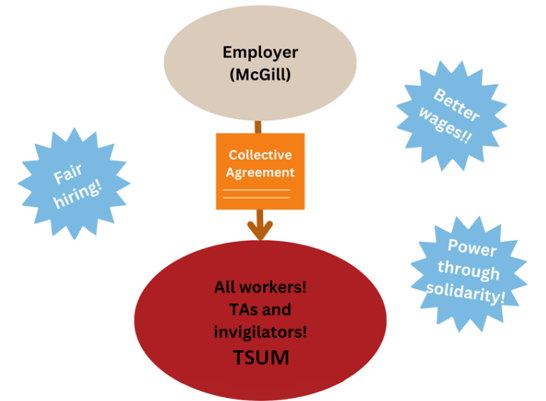
\includegraphics[width=1\linewidth]{Pictures/tsum1.png}
        \caption{How TSUM works.}
        \label{fig:img1}
    \end{subfigure}
    \hfill
    \begin{subfigure}[b]{0.48\textwidth}
        \centering
        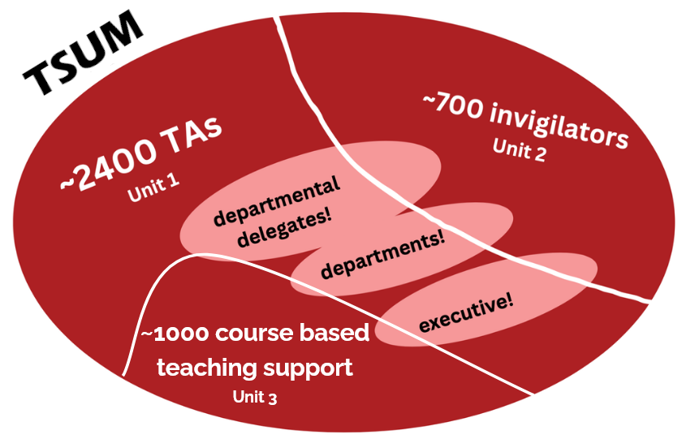
\includegraphics[width=\linewidth]{Pictures/tsum2.png}
        \caption{Members of TSUM.}
        \label{fig:img2}
    \end{subfigure}
    \label{fig:both_images}
\end{figure}

 \noindent The union\textbf{ negotiates on your behalf }and enforces collective agreements with McGill to establish standardized wages, working hours, benefits, and priority rights. The union also defends workers against unfair labor practices, tracks cumulative hours and overtime, and helps members address workplace disputes.

\noindent \textbf{\sffamily What is a Delegate?} \index{TSUM!Delegate}\\
Delegates are your union representatives at the departmental level. Delegates are also your \href{https://mgaps.physics.mcgill.ca/people}{\textbf{first points of contact}} in your union! Delegates engage with TAs in their department via emails, phone calls, and office visits. They also check the tentative hiring list every term to ensure the worker hiring rights are respected and also assist you in filing grievances. In addition, they serve on the Delegate’s Council to assist in union governance. 

\noindent The Physics department currently has 3 delegates. You can contact them via email: \url{https://tsum-stsem.ca/contact/}. \\


\noindent \textbf{\sffamily What else do we do?} \\
We fight for better working conditions through prioritizing regular, meaningful engagement with all of our members. We do this by: 
\begin{itemize}
    \item \textbf{General Assemblies:} TSUM hosts general assemblies \textbf{once per term} and unit assemblies once per year where we discuss workplace issues and solutions and vote on things like bargaining and negotiations, union finances, and leadership. You also get a free meal paid for by the Confédération des Syndicats Nationaux (CSN), our parent labour union! \\
    \item \textbf{Bargaining}: We are currently in the process of pre-bargaining with McGill to renew our CA that is set to expire on July 31, 2027. Regular updates, will soon be available on this \href{https://tsum-stsem.ca/news/}{link.}  \\
    \item \textbf{Grievances:} TSUM solves any disputes that may arise between the university and an employee such as late pays, going over contract hours, unsafe working conditions, etc. To file a grievance, reach out to a delegate or a \href{https://tsum-stsem.ca/your-rights/grievance-frequently-asked-questions/}{TA grievance officer}. \\
    
    \end{itemize}

\noindent \textbf{\sffamily What can you do?}\\
To help our cause you can do the following things: \\
    \begin{enumerate}
    \item \textbf{Sign the \href{https://tsum-stsem.ca/members/membership-forms/}{membership form}.} All TAs are considered members of the union whether or not they sign the card or not, however, if less than 50\% sign the card, the union would require a vote to be certified. Hence, it is highly recommended to sign you card as soon as you become a TA to ensure that the union maintains its strength.  \\ 
    
    \item \textbf{Attend Assemblies}, social gatherings such as rallies, potlucks, BBQs etc. Since TSUM is a democracy, assemblies are where we make major decisions that affect all members of the union. Make your vote count! \\
    
    \item \textbf{Get involved:} TSUM has several open positions in various commitees and working groups. You can also become a \textbf{delegate} or run for an executive position. To become a Physics delegate, you need to nominate yourself at the MGAPS Fall Assembly. \href{https://docs.google.com/forms/d/e/1FAIpQLSd1uaNmDgvsz2AEtq9MbR7N8De4p6-33g2jSGqGDNHRUkmbfA/viewform}{Here's} a general interest form that you can sign if you wish to be involved in mobilization, communications or other TSUM activities.\\
    
    \item \textbf{Bargaining:} Since this year is bargaining year, you can also get involved with the bargaining commitees. Did you know that you can also attend \textbf{open bargaining} sessions between the union and McGill and witness the negotiations in real-time? Stay glued to your email for more information.\\
\end{enumerate}

  \begin{plainexercise}
        \textbf{TA training:} All \textbf{\underline{first time TAs}} get up to 3 hours of paid teaching training, in addition to your contract hours! The training is organized by the Teaching and Learning Services (TLS). To know more, follow this \href{https://www.mcgill.ca/teaching-academic-programs/instructors/programming/ta-training}{link}.
    \end{plainexercise} 


\subsection{Extra hours for TA}   
    In the event that you work over your allotted 90 hours per semester you may request more paid hours from your course supervisor. Your contract guarantees that you get paid for 90 hours of work, so you will at a minimum always get paid for 90 hours of work. 

    Keep track of your hours each week in order to know if you are being over worked. If you do go over hours and don't want to work anymore you don't have to! For any unfinished work the university must offer you the hours required at the TA rate before they are offered to anyone else. But you are under no obligation to accept this offer.

    If your additional hours are no approved you stop working. You cannot be asked or expected to complete free work for the university. If your course supervisor tries to force you to work for free or if your TA work is outsourced to a non TA contact your delegates or TA officer immediately as this is a violation of your rights as a worker.

\section{How to be a Good TA?}
\subsection{Grading}
Grading is one of the most essential TA tasks. Most of your working hours will be spent grading assignment and exams. It is a very good idea to communicate with the instructor early to establish guidelines. Some instructors are very lenient with grading while others have strict guidelines. Regardless, the most important thing is to be \textbf{consistent.} \vspace{5pt}

\begin{itemize}[leftmargin=10pt]
    \item \textbf{Design a good grading rubric.} Spend enough time to make it useful and stick to it. Once you are done grading, give the rubric to the students so that they can verify their solutions.
\end{itemize}
\begin{plaincorollary}
    Quite often, you will need to retroactively change your rubric based on the first few evaluations. That's perfectly fine! Make sure that you go back and grade everyone fairly.
\end{plaincorollary}
\begin{itemize}[leftmargin=10pt]
    \item \textbf{Provide useful feedback.}  Mention explicitly where marks have been lost and the point total per question. All feedback should define the actions a student can take to improve themselves. Make a list of common errors and communicate them to the class in tutorials.\\
    \item In case of \textbf{late submission}, you may contact the student via email and ask for justification. Typically, it's okay to accept late submissions, especially in case of illness or travel or if the student has had prior permission from the instructor. However, the final decision rests at the discretion of the course instructor.\vspace{5pt}
\end{itemize}
\begin{plainexercise}
If you stumble upon \textbf{plagiarized} content, work that's clearly unoriginal, contact the instructor immediately. This is well above your pay-grade as TAs are not expected to deal with such serious offences. 
\end{plainexercise}

\subsection{Tutoring/Office Hours}
Tutorials and office hours are useful for students to get in-depth feedback and ask questions. They also enables you to develop better communication skills.

\begin{itemize}[leftmargin=10pt]
\item \textbf{Spend time} reviewing the concepts and questions a day before. Try solving the problems atleast once without looking at the solutions. \\

\item When solving a problem in class, write each step carefully and legibly and ask students for \textbf{constant feedback} on whether they are able to follow the procedure or whether a particular formula has been taught in class. \\

\item You can always \textbf{divide the class into groups} to work on problems if you wish. You can also ask students to analyze a certain calculation when they go back home if you don't have time to go through it in class. \\

\item During office hours, if students don't have any particular questions, you can go over \textbf{previous quizzes or exam problems}. \\
\end{itemize}

\begin{plaincorollary}
    Students may often ask you questions that you are not prepared for. Don't Panic! You are not the one being tested on your knowledge. Just tell them that you'll get back to them via email or during next class.
\end{plaincorollary} 


\subsection{Labs}
Labs are important opportunities for students to apply their knowledge and gain experimental
skills. It's your responsibility as a lab TA to ensure that students stay on the right track while also letting them learn experimental practices though trial and error. 
\begin{itemize}[leftmargin=10pt]

    \item Ask the instructor for \textbf{clear instructions} and rely on the rubric rather than your own intuition.\\

    \item \textbf{Read} through the entire lab manual or protocol ahead of time and test out calculations or tricky steps.\\
    
    \item \textbf{Communicate objectives} not only with your course supervisor, but also your fellow TAs who will be facilitating the lab with you. \\

    \item \textbf{Use your own experience} as a student to recognize common pitfalls and sources of errors. \\
    
    \item Do not just giveaway the answers to students' questions. However, if you see them struggling, don't wait, 
    \textbf{be proactive} and offer them the necessary help.\\
    \item Make sure that students are aware of universal \textbf{lab safety rules} and ensure that students are not fooling around with equipment, especially instruments that involve electricity.    
\end{itemize}

\begin{plainexercise}
    Always remember to create an \textbf{inclusive} space where students feel comfortable asking questions and sharing their problems. Let them know that there are no silly questions!
\end{plainexercise}

\section{What is the TA Wiki?}\index{TA Wiki}
The \href{https://wiki.hep.physics.mcgill.ca/TAWiki/index.php?title=Main_Page}{TA Wiki} is a brand new initiative undertaken by MGAPS. The purpose of the wiki is to improve continuity between semesters, overcome institutional memory loss, and provide a common space for organizing \textbf{TA-related information and expected responsibilities}. It can be used for the following purposes:
\begin{itemize}
    \item \textbf{TA Hour Logging:} tracking the number of hours worked throughout a semester to maintain transparency for workload. \\
    \item \textbf{Task Breakdown and Expectations:} including descriptions of expected TA duties and recurring responsibilities. \\
    \item \textbf{Information for Future TAs:} for applying to specific TA positions and course-specific tips and recommendations. 
\end{itemize}

\begin{SCfigure}[2][hbt]
    \centering
    
\includegraphics[width=0.3\linewidth]{Pictures/Wikisignup.png}
    \caption*{Since the initiative is in its infancy, we need your help to complete the TA wiki! Just sign up for it and record your experience at the end of the semester. \\

    \textbf{\color{ocre} Note:} You need to make an account to access and edit information on the site. Account creation is currently only possible with admin privileges. Reach out to one of the TSUM delegates or the RTech officer to make an account or simply fill this \href{https://docs.google.com/forms/d/e/1FAIpQLSfjcshi98m5lyCXsSaB7t7WEa-NcOw9MPB3S9mSrw_FOCMVWQ/viewform}{form}. \\
    
    To learn more about the initiative, follow these \href{https://wiki.hep.physics.mcgill.ca/TAWiki/images/f/fd/TAWikiGuide.pdf}{slides.} }
    \label{fig:TAwikisignup}
\end{SCfigure}

\section{Are there non-TA positions?}
If teaching is not your cup of tea, then there are other jobs in the department that you can apply to instead. The pay is equivalent to that of a TAship with a one-year or one-semester long commitment. \\

\noindent \textbf{\sffamily EDI Committee}\index{Coordinators!EDI}\\
The EDI graduate coordinator serves on the EDI committee. The EDI committee strives to make our department workplace more equitable and inclusive. They facilitate ongoing efforts (such as our CEGEP workshops, the Contemporary Physicists website, and others) as well as provide administrative support (such as meeting organization). Additionally, the coordinator also helps the committee organize events such as once-to-twice-a-semester social events and an EDI colloquium. Typically \textbf{1-2 positions} are available each year. \\

\noindent \textbf{\sffamily Outreach Committee}\index{Coordinators!Outreach}\\
The Outreach Coordinators are members of the \href{https://physics-tsi-outreach.physics.mcgill.ca}{Physics \& Trottier Space Institute (TSI) Outreach Committee}. The coordinators work alongside and receive support from the committee, which meets regularly to plan, schedule, and organize our outreach events. There are currently 4 student coordinator positions across the two departments: Hackathon (Physics), Public Talks \& SciComm (Physics), Space Explorers (TSI) and Science in Space (TSI). \\

\begin{itemize}[leftmargin=10pt]
    \item \textbf{Hackathon Coordinator} \index{Coordinators!Hackathon} is responsible for organizing and delivering the annual Physics Hackathon, with support from the Outreach Committee. The coordinator's main responsibilities include: planning and coordinating the weekend-long event, securing sponsorships, and training and recruiting volunteers, mentors, and judges.
\begin{figure}[hbt]
    \centering
    
\includegraphics[width=0.7\linewidth]{Pictures/Hackathon.png}
    \label{fig:hack}
\end{figure} \\
 \item \textbf{Public Talks \& Science Communication Coordinator} \index{Coordinators!Public Talks} organizes public talks and creates content for social media and the outreach website. The coordinator's main tasks are recruiting speakers for the monthly talks, finding venues, advertising talks, coordinating volunteers, and creating and posting content to Physics social media accounts.\\

\item \textbf{Space Explorers Coordinator} \index{Coordinators!Space Explorers} is responsible for running the Space Explorers program, which brings fun, inquiry-based activities to elementary schools throughout Montr\'eal. They must recruit, communicate with, and train volunteers to deliver the program in schools and coordinate with schools to schedule visits. \\

\item \textbf{Science in Space Coordinator} \index{Coordinators!Science in Space} organizes and manages the Science in Space program in which middle school students of under-represented genders in physics build telescopes in Minecraft over a period of \~10 weeks. They are expected to deliver hands-on lectures and coordinate with schools to schedule visits. 
\end{itemize}

\noindent In addition, there are other jobs outside of the department you can apply through Workday as a replacement for TAship. 

\section{More FAQs?}
\begin{itemize}[leftmargin=10pt]
    \item \textbf{Where can I read more about good TA practices?} \newline
    You can refer to the previous  \href{https://mgaps.physics.mcgill.ca/files/Physics-TA-Handbook.pdf}{MGAPS TA Handbook} compiled by Benjamin Dringoli for more knowledge. Despite being a more than few years old, you'd find the content to be very useful.\\
    \item \textbf{Where can I turn for support as a TA and a graduate student?} \vspace{5pt}
    \begin{itemize}
        \item Teaching and Learning Services McGill:\url{www.mcgill.ca/tls}
        \item The Labour Union (TSUM): \url{https://tsum-stsem.ca/}
        \item SKILLSETS McGill: \url{http://www.mcgill.ca/skillsets/offerings/ta-trainings}\\
    \end{itemize}
    
    \item \textbf{Who do I reach out to in case of disputes?} 
    The TSUM delegates are the \href{https://mgaps.physics.mcgill.ca/people}{\textbf{first points of contact}} if you have any questions. Depending on your specific case, they'll forward your complaint to the respective authority. See \href{https://tsum-stsem.ca/your-rights/grievance-frequently-asked-questions/}{this} page for more details. \\
   
    \item \textbf{How much tax do I pay?}\index{Taxes!TA Salary}\\
    The TA stipend is taxable and the amount of tax depends on the duration you have TAed for. Some of the amount is non-refundable but you could get back $\sim \$100-\$200$ when you file taxes at the end of the year. Here's a short overview of what taxes you pay on your stipend as of 2026:
    \begin{itemize}
        \item \textbf{Union Dues:} 2.5\% (non-refundable)
        \item \textbf{Employment Insurance (EI):} 1.3\% (non-refundable)
        \item \textbf{Provincial Parental Insurance Plan (PPIP):} 0.43\% (non-refundable)
        \item \textbf{Quebec Pension Plan (QPP):} exempt up to \$3500, thereon 6.3\% (refund depending on your gross income).
    \end{itemize}
    
    %\item \textbf{Auto deposit?}

\end{itemize}
